\documentclass{article}
\usepackage[round]{natbib}
 
\usepackage{graphicx}
\usepackage{authblk}
\usepackage{amsmath}
\usepackage{graphicx}
%\usepackage[margin=0.85in]{geometry}
\usepackage[margin=1in]{geometry}
\usepackage{lineno}
\usepackage{float}
\usepackage{cleveref}
\usepackage{tabularx,ragged2e}
\usepackage{url}
 
\usepackage{inputenc}
\renewcommand{\baselinestretch}{2.0} 
 

\newcommand{\source}[1]{\hfill Source: {#1}} %command definition for sources in figures

\title{Evaluating statistical modeling of Nitrogen Dioxide using air quality sensors onboard a carrier bicycle}
\author{Meng Lu,  Ruoying Dai,  Cjestmir de Boer, Ingeborg Kooter, Oliver Schmitz, Simona Cristescu , Derek Karssenberg}
\date{\today}
%[1] Department of Physical Geography, Utrecht University, Princetonlaan 8a, 3584 CB, Utrecht, the Netherlands \\
%[2]Netherlands Organization for Applied Research, TNO, Princetonlaan 6, 3584 CB, Utrecht, the Netherlands \\
%[3] Institute for Molecules and Materials, Radboud University,
%Heyendaalseweg 135, 6525 AJ Nijmegen, the Netherlands

\begin{document}

\maketitle

\begin{abstract}
Statistical learning models have been applied to study the spatial patterns of ambient Nitrogen Dioxide (NO$_2$), which is a highly dynamic, traffic-related air pollutant. However, the validation process in most studies is based on split-sampling of observations from fixed ground stations, mostly sparsely distributed over a region or country. This implies that validation does not consider how well models are capable of representing spatial patterns in air pollution mostly occurring over distances shorter than the ground station sampling spacing. This may lead to inadequate hyperparameter optimisation and bias when comparing between different statistical models. External mobile measurements are therefore needed for more reliable model evaluations as these provide detailed and spatially continuous information on air pollution patterns. However, most current designs of mobile NO$_2$ sensing data sets do not fulfill all requirements for validation, in particular: 1) spatially detailed coverage of NO$_2$ measurements in areas of interests (e.g. along streets, city centres, and residential blocks, which may not be accessible by auto-vehicles); 2) sufficient repetitions over time so that the measurements are representative to concentrations over a relative long-term period; and 3) collected with high-end sensors on-board (they are commonly too heavy to be carried by a person). In this study, we installed a mobile air quality station on-board  a cargo-bike to collect data that meet these requirements. The collected data is then used for a more in-depth understanding of the statistical modeling of NO$_2$. We found that our cargo-bike measurements provide useful additional information compared to bootstrapped validation solely based on ground station measurements. The statistical model comparison results differ considerably between only considering ground stations for validation and additionally including the external validation dataset. 

 
\end{abstract}

\section{Introduction}
Chronic exposure to air pollution poses a threat to public health. The World Health Organisation estimated air pollution to contribute to 7 million deaths worldwide in 2016 \citep{world2018burden}. From a medical perspective, common air pollutants such as particulate matter and nitrogen oxide (NO$_2$) damage the cardiovascular and respiratory systems \citep{anderson2012clearing, pascal2009effets}.  In the Netherlands, the NO$_2$ concentration limit set in 2017 was exceeded for several times in areas with busy traffic\citep{no2}. Emissions from traffic can be direct and indirect. Atmospheric NO$_2$ is mostly traffic-related as an indirect secondary emission of an oxidation result of emitted NO, while the direct primary emission as NO$_2$ is minor \citep{ukno2,no2}. Quantifying NO$_2$ is crucial for interventions to abate exposures.

 Ground monitoring stations of NO$_2$ can be routinely run or are project-oriented, which involves considerable investments \citep{hoek2008review}. Recent studies show a rise in urban low-cost ground sensors providing additional information to increase the level of detail in spatio-temporal mapping \citep{spinelle2015field, schneider2017mapping,isiugo2018assessing}. Low-cost sensors can provide additional information to satellite and regular ground monitors in particular enabling higher-resolution mapping of air pollution in space-time. Meanwhile, the deficits of low-cost sensors are noted as well. Measurements from low cost sensors are subject to sensor drift and interference effects. Sensor drift denotes the growing bias of sensor response due to the ageing electrochemical cell; interference effects, i.e. the sensor's response to other pollutants, gases, temperature and relative humidity, hampers the measurement of the target pollutant \citep{van2019calibration}. For instance, an application of low-cost sensors in the Netherlands carried out in Amsterdam showed a significant signal drift over a time span of two months. Calibration with temperature and relative humidity however improved the fit with ground stations \citep{mijling2018field}. 
 
Methods for spatiotemporal mapping of NO$_2$ include dispersion models \citep{holmes2006review, health2010traffic}, statistical models \citep{chen2019comparison}, or hybrid models \citep{molter2010modelling,marshall2008within,beelen2010comparison,dijkema2010comparison, akita2014large}. Dispersion models simulate the emission, transformation, transportation, and deposition of atmospheric particles, but require detailed emission inventory data and are computationally intensive; scaling a dispersion model towards larger areas can be at the cost of computational intractability. Statistical models aim at finding relationships between ground monitor station observations, satellite measurements, and ancillary NO$_2$ data, called geospatial predictors \citep{rivera2013nitrogen, park2017individual,kharol2015assessment, isiugo2018assessing, chen2019comparison,luglobal}. The geospatial predictors are variables that relate to the emission sources (e.g., transport network) and dispersion processes (e.g., meteorological data) of the pollutants \citep{briggs2000regression}. The approach has been used to predict high-resolution NO$_2$ at various spatial scales \citep{Hoek2008,larkin2017global} and is the focus of this study.  Recently, mapping temporally resolved, long-term NO$_2$ climate, e.g. NO$_2$ of each hour of a day aggregated over multiple years \citep{lu2020land}, has been shown to be preferable to account for human space-time activities in personal exposure assessment \citep{lu2019}. However, validation thus far is mostly done against ground station measurements, which does not enable extensive validation of the spatial pattern of air pollution predictions. To validate spatiotemporal predictions regarding spatiotemporal patterns, external measurements providing more detailed spatiotemporal information are necessary.

A spatially continuous ground validation dataset is also essential for evaluation and comparison of different statistical models. A wide array of models have been developed using a single or a stack of linear regression \citep{briggs2000regression} or machine learning models \citep{kees2020satelliteML}. Several studies compared the accuracy of high resolution NO$_2$ mapping of various statistical models, including standard and regularised linear regression, ensemble tree-based models, transformation-based (e.g. support vector machine), artificial neural networks \citep{chen2019comparison, kerckhoffs2019performance, luglobal}. \cite{kerckhoffs2019performance}, modelling UFP (Ultra Fine Particles), and \cite{chen2019comparison}, modelling NO$_2$ of several European countries, obtained similar validation accuracy across various ensemble tree-based and linear regression models. Based on the validation accuracy comparison results, they concluded that various statistical algorithms obtained similar performance. However, neither of these two studies showed or validated the prediction patterns. Also, in the global NO$_2$ modelling study of \cite{luglobal}, it is found that various ensemble tree-based methods obtaining almost the same accuracy based on Cross Validation on Ground Stations (CVGS) may give very different prediction patterns.  
%to what extent can the CV prediction accuracy indicate the spatial variation modelled? 

The goal of this study is to 1) design a study to collect such spatially continuous observations of air pollution, and 2) use it to further evaluate and compare statistical NO$_2$ models built using an official national ground air quality monitoring network. In particular, we will answer the question whether, with spatially continuous observational data we can better optimise hyperparameters in the models used and whether model comparison results differ from those based on CVGS?

%\begin{enumerate}
%    \item How can we collect spatially continuous data that provide small-scale NO$_2$ variations?
%    \item If we validate models on this data, are the model comparison results differ from evaluating %based on CV on stations, for high resolution mapping?  
%\end{enumerate}

We monitor NO$_2$ concentrations by installing a mobile air quality station on-board a cargo-bike to evaluate temporally resolved NO$_2$ models based on different statistical algorithms. Specifically, we focused on comparing three methods, Lasso \citep{lasso}, Random Forest \citep[RF,][]{breiman2001random}, and extreme gradient boosting \citep[XGBoost, XGB,][]{xgboost}. These methods are selected as they are representative for the most recent spatial prediction techniques for NO$_2$ mapping, with Lasso and Random Forest compared in \cite{chen2019comparison, kerckhoffs2019performance, luglobal}. We compared the Lasso, RF, and XGB models of the corresponding hours with the cargo-bike measurements to understand the amount of spatial variability a statistical model could capture, and to compare different models and hyperparameter settings beyond CVGS accuracy of the models. %The implications can be generalised to comparing other statistical methods.    %and to imply a validation method that accounts for spatial prediction patterns.  



\section{Data}

\subsection{Cargo-bike and instruments}


The cargo-bike was designed to carry reference apparatus in a compact package, to operate with optimal freedom of movement while providing reliable measurement data. It was equipped with two 12,8V/100Ah LiFePo4 batteries (Victron), a high efficiency MultiPlus Compact inverter/charger (Victron) and a 150Wp solar panel. 
The cargo-bike and the instruments on board weights 160kg, has an e-bike support motor and can operate 3-5 hours continuously.
% It carries a 150 WP solar panel and can work 3 – 5 hours continuously.   

The air quality monitoring apparatus were: 42i NO$_x$ monitor, 49i O3 monitor (Thermo Fisher Scientific), model 3321 APS (TSI), WXT536 climate sensor (Vaisala), MI70 + probe GM70 CO2 sensor (Vaisala), GPS, a PC and several low-end air quality sensors. The housing was custom made from sandwich panel and extruded aluminium profiles. 

The cargo-bike covered a route shown in \cref{route}, in Nijmegen, the Netherlands, from July 16 to 19, 2019. The total route length is 29 km. The cargo-bike measured NO$_2$ every morning from 8 am to 11 am, the route was repeated daily. A two-point calibration was performed on the Thermo 42i NO$_x$ monitor using synthetic zero gas (0 ppb) and calibration gasses of NO (410 ppb) and NO$_2$ (366 ppb). After calibration, the sensed NO$_2$ averaged over the four days have a mean of 11.21 $\mu g/m^3$. The cargo-bike measurements are aggregated in space-time to every minute, and aggregated over the four days, to eliminate effects from random vehicles to represent general emission patterns.    



\begin{figure}[H]
    \includegraphics[scale = 0.8,trim=1cm 0cm 3cm 2cm, clip=true]{f1a.jpg}
    
    \caption {The cargo-bike and instruments that are used to sensor the NO$_2$ in our study.}
    \label{bike}
\end{figure}

\begin{figure}
    \includegraphics[width=\linewidth,trim=4cm 1cm 4cm 1cm, clip=true]{f1b.jpg}
    
    \caption {Routes taken by the cargo-bike, the background map is from OpenStreetMap\citep{openstreetmap}. The starting and ending locations are the same, indicated by the point "A". }
    \label{route}
\end{figure}
%“A” indicates the starting point.The point numbers indicated on the map are used to indicate the routes. For example route from point 1 to point 2, which is called route 1-2 in this study.

\subsection{Ground monitor stations used for statistical modelling}

In the Netherlands (41,543 $km^2$), 66 ground stations are established and are managed by the National Institute for Public Health and the Environment \citep[RIVM,][]{RIVMLML}. We further incorporated the ground monitor network from Germany (376 stations 357.386 $km^2$) to better identify NO$_2$-predictors relationships using machine learning models. The ground monitoring station measurements are from the European Environment Agency \citep{EEA} for the Netherlands and the Umwelt Bundesamt \citep{germansource} for Germany. Three stations with inadequate measurements (i.e. missing values at certain hours) are neglected. The measurements are downloaded for the same days as the cargo-bike measurements and from 7:00 am - 11:59 am.  

The ground station measurements used for prediction are aggregated in two ways, one is the mean of all hours and days measured by cargo-bike, called NEDL-avg dataset, and the other the mean of each hour of the days corresponding to the time of cargo-bike measurements, called NEDL-hr dataset. The NEDL-avg is used for XGB and RF hyperparameter optimisation. The NEDL-hr is used for building and validating the statistical models.
%and different hyperparameter settings with the cargo-bike measurements.  

In Nijmegen, where the cargo-bike took the measurements, there are two ground stations established, one is the Nijmegen-Graafseweg station (called Graafseweg station, Latitude: 51.941372, Longitude 5.857777), which monitors mainly air pollution from traffic. The other is Nijmegen-Ruyterstraat station (called Ruyterstraat station, Latitude: 51.838221, Longitude: 5.856938), which monitors mainly background pollution. The stations are managed by RIVM. Over the period of the cargo-bike measurements considered, the mean NO$_2$ level is 23.25 $\mu g/m^3$ and 14.03 $\mu g/m^3$, respectively, for the Graafseweg and the Ruyterstraat stations.  

\subsection{Geospatial predictors}
 The geospatial predictors (\cref{tab:prevar}) were calculated at 25 m resolution. They are either spatial attributes aggregated within a circular ring centred at each sensor or prediction location, called buffered predictors, or values of the spatial attribute at the observation or prediction location, called gridded variables. The buffered predictors include industry areas, roads, VIIRS (Visible Infrared Imaging Radiometer Suite) Nighttime Day/Night Band (DNB) radiance values \citep[nightlight,][]{nightlight} and population. Gridded variables include wind speed and temperature \citep{dee2011era}, elevation \citep{amante2009etopo1}, TROPOMI level 3 product of NO$_2$ column density from 2019-01 to 2019-12. 
 %OMI level 3 product of the 2017 annually aggregated NO$_2$ vertical column density, and the GEOS-CHEM \citep{bey2001global,GEOS-CHEM} annual NO$_2$ surface concentration product \citep{geddes2016long} of 2013. 
We used the TROPOMI NO$_2$ measurements from 2019 due to the fact that the measurements are available at higher spatial resolutions ($3.5 \times 7 km^2$, $3.5 \times 5.5 km^2$ since 06, August, 2019). The buffered predictors of road and industry are calculated from OpenStreetMap  \citep{openstreetmap}. For detailed descriptions of the sources of geospatial predictors and how they are calculated please refer to \cite{luglobal}.   
  
  
\begin{table}[H] 
\centering
\caption{Predictors used in this study. "\_mon" indicates months, (mon = 1,...,12).  "\_buf" indicates the buffer radius for road density and industry areas. The buffered predictors with buffer radii of 25 m, 50 m, 100 m, 300 m, 500 m, 800 m, 1000 m, 3000 m, 5000 m are calculated. "\_bufnl" indicates the buffer radius for the nightlight. The buffer radii of 450 m, 900 m, 3150 m, 4950 m, are calculated. The original resolution is provided for gridded (raster) variables and data types for vector variables.}

\label{tab:prevar}
{
\begin{tabular}{p{6cm}|l|l|l}
\hline
Predictor                                    & Variable name                & Unit         & Resolution /data type         \\ \hline
Monthly wind speed at 10 m altitude. &  Wind\_speed\_10m\_mon   & km/hr         &    10 km \\ \hline
Monthly temperature at 2 m altitude.  & temperature\_2m\_mon  &  Celsius        &    10 km \\ \hline
%OMI 2017 annual mean vertical column density. & OMI\_mean\_filt; OMI &  $mol /cm^2$ &    0.25 arc degrees \\ \hline
 
TROPOMI 2019/01 - 2019/12 mean vertical column density.  & trop\_mean\_filt; Tropomi&  $mol /cm^2$ &   0.01 arc degrees  \\ \hline

%Remote sensing product generated of 2011 from \cite{geddes2016long} & RSp &$\mu g/ m^3$ & 10 km \\ \hline
Population in 5 km grid  & population\_5000 & count  & 5 km \\ \hline
Population in 3 km grid & population\_3000 & count  & 3 km \\ \hline
Population in 1 km grid  & population\_1000 & count  & 1 km\\ \hline
Nightlight  & nightlight\_bufnl & $W cm^{-2} sr^{-1}$  & 500 m\\ \hline
Total length of highway  & road\_1\_buf  & m &polygon, lineString              \\\hline
Total length of primary roads                   & road\_2\_buf          & m  &polygon, lineString            \\\hline
Total length of local roads     & road\_M345\_buf        & m  &polygon, lineString               \\\hline
Area of industry                                    & I\_1\_buf           & m$^2$ &polygon, lineString            \\\hline
 

\end{tabular}
}  
\end{table}

\section{Methods}

\subsection{Research Design}
The methodological framework is designed as follows: 
\begin{enumerate}
    \item A set of statistical learning methods are applied to model hourly NO$_2$ from official ground station monitors. These statistical learning models are compared. The variable importance calculated in these methods are used to identify the mapping resolution. 
    
    \item Hourly NO$_2$ are predicted for the study area with each of the statistical models and are validated on the continuous measurements from the cargo-bike.
    
    \item The measurements from the cargo-bike are used to compare predicted patterns from hourly XGB models with different hyperparameter settings. 
    
\end{enumerate} 


%\subsection{Spatial stationarity and dependency}
%We used GWR (Geographically Weighted Regression) to explore local variability of ground station measurements and found no significant location variability from the errors, weights, and R-squared ($R^2$) of the GWR model.  This ensures adding ground stations from Germany will not contribute negatively to the model. The spatial correlation is tested by calculating variograms with various cut-offs. It is found that station measurements can be treated in the modelling and validation process as spatially independent observations.


\subsection{Random Forest, Extreme Gradient Boosting, Lasso}

Lasso is a linear regression algorithm that uses an L1 norm to shrink variable coefficients to zero to reduce model variance. RF and XGB are ensemble tree-based methods, which mitigate two negative effects of a single tree model: instability and coarse separation. Large trees are subject to instability, while small trees are inaccurate for their piece-wise constant approximations. Bagging overcomes these two constraints by using small trees to add stability and avoid coarse approximation by averaging over small trees \citep{friedman2001greedy}. RF is based on Bagging, which grows trees independently while XGB is based on gradient boosting, which grows trees subsequently based on current model residuals. RF extends from bagging by choosing the variable to split from a subset a number of variables. XGB is a scalable gradient boosting algorithm, which enables multiple penalisation paths to control model complexity to prevent model over-fitting, including regularisation on tree width and terminal node values, as well as dropping trees.  

The variable importance is calculated for XGB and RF. We use the averaged ranking in 20 times bootstrapping for each method \citep{luglobal}. For the XGB the gain scores \citep{chen2016xgboost} are used and for the RF the permutation test is used to calculate the variable importance. 


\subsection{RF and XGB hyperparameter optimisation}

The NLDE-avg dataset is used for hyperparameter optimisation, through grid search, with 5-fold CVGS. For XGB, the learning rate (eta), number of iterations (rounds), maximum tree depth (max.tree.depth) and gamma are tuned, each time 70\% of data is drawn from the training set. The search grid for the number of iterations (rounds) was from 200 to 3000, with a step of 200; maximum tree depth (max-depth) from 3 to 6 with a step of 1, learning rate (eta) from 0.001 to 0.1 with a step of 0.05, the penalty term gamma \citep{xgboost} from 1 to 5 with a step of 1. The 5-fold CVGS result indicates the optimal hyperparameters to be eta = 0.051, rounds = 200, max-depth = 3, gamma = 1. For RF, the minimum number of trees on the end nodes (min.node.size), and number of variables that are randomly drawn for each tree (mtry) are optimised. The optimal setting for RF is min.node.size equals 5 and mtry equals 12, the number of trees is set to 1000 for random forest, which is a safe choice as the high number of trees will not negatively affect model performance.
 


\subsection{High setting of XGB hyperparameters}
As the spatial pattern of XGB can vary greatly with different hyperparameter settings despite the CVGS accuracy remaining the same \citep{luglobal}. We evaluated results from multiple XGB hyperparameter settings. We tested increased learning rates of 0.002, 0.001, and 0.0005, and estimators (i.e. the number of trees) of 300, 3000, and 5000. We found altering the learning rate from 0.002 to 0005 only affect the prediction patterns subtly but setting the learning rate to 0.002 and 0.051 (original setting optimised by CVGS) makes a considerable difference in their predicted NO$_2$ patterns. The CVGS accuracy is optimised at 3000 trees with this new learning rate, which remains approximately the same compared to the original setting (\cref{cv-hr}). We also increased the L1 norm (lambda) from 2 to 10, with a step of 2, and gamma \citep{chen2016xgboost} to 5, to further control respectively extreme values at the terminal node and model complexity. With these settings the spatial prediction patterns of XGB, as well as their correlations with cargo-bike measurements change subtly. We will show the result of XGB with the maximum tree depth setting to 5, learning rate 0.002, number of estimators 3000, lambda 2, and gamma 5. We refer to this hyperparameter setting of XGB as "high setting" (XGB hs); compared to the original setting, it searches the gradient much more slowly, correspondingly with more iterations, and uses additional penalties to control model over-fitting. 

 
\subsection{Accuracy assessment}

The RMSE (Root Mean Squared Error) provides general insight into the variance and magnitude of the error. In addition, we calculated the MAE (Mean Absolute Error) for the magnitude of the error and the IQR (Inter-Quartile Range) for the variance of the error. To make the accuracy assessed at different times comparable, we calculated the R-squared ($R^2$). We used 80\% of the dataset for modelling and 20\% for validation. A 20-time bootstrapped Cross-Validation was used. Thus the accuracy metrics described above were calculated on validation datasets 20 times, and the median of each was used as the final accuracy measure.    

 
%%%%%%%%%%% 
% Results %
%%%%%%%%%%% 

\section{Results}
\subsection{Models trained on NLDE-avg}

\Cref{nlde_vimp} compares the variable importance obtained by the RF and XGB models trained on the NLDE-avg dataset. The top three ranked variables are the same, including the emission-related variables primary road length within 25 m buffers. This indicates the maps can capture spatial variability at 25 m resolution. Therefore, the statistical modelling is based on 25 m resolution grids. Other emission-related variables include primary roads in 50 m and 100 m buffers and local roads in 100 m buffers. The variables are ranked similarly between RF and XGB. 
%Compared to the RF, the XGB predictions appear to be more strongly related to the road pattern, evidenced by the selection of the 50 m buffered variable of the local road length. 
The mean predictions ($\mu g/m^3$) along the cargo-bike track are 18.8 for XGB, 20.0 for RF, and 19.2 for Lasso. Over the study area, the Pearson's correlation coefficients between XGB and RF predictions is 0.97, between RF and Lasso 0.94, XGB and Lasso 0.90.

% The $R^2$ of XGB, RF, Lasso against cargo-bike measurements are respectively 0.06, 0.08, and 0.05, calculated over the predictions at the 25 m cells corresponding to the cargo-bike track. The CVGS (\cref{nlde_cv}) result indicates that RF and XGB have a similar performance, and they both outperform Lasso. 
%In many areas. the XGB model predicted higher values compared to the RF and Lasso predictions and the cargo-bike measurements (\cref{maps}). 
 
\begin{table}[H] \centering 
  \caption{Ranking of the top 15 most important variables of XGBoost and Random Forest, using NLDE-avg. Please refer to  \cref{tab:prevar} for the variable description.} 
    \label{nlde_vimp} 
\begin{tabular}{@{\extracolsep{5pt}} ccc} 
\\[-1.8ex]\hline 
\hline \\[-1.8ex] 
Rank & XGBoost & Random Forest \\ 
\hline \\[-1.8ex] 
1 & population\_3000 & population\_3000 \\ 
2 & road\_class\_3\_3000 & road\_class\_3\_3000 \\ 
3 & road\_class\_2\_25 & road\_class\_2\_25 \\ 
4 & radiation & population\_5000 \\ 
5 & population\_1000 & road\_class\_2\_50 \\ 
6 & population\_5000 & road\_class\_3\_5000 \\ 
7 & road\_class\_2\_100 & road\_class\_2\_100 \\ 
8 & road\_class\_3\_5000 & population\_1000 \\ 
9 & road\_class\_2\_50 & nightlight\_3150 \\ 
10 & nightlight\_450 & elevation \\ 
11 & elevation & wind\_speed\_10m\_9 \\ 
12 & road\_class\_1\_5000 & nightlight\_450 \\ 
13 & trop\_mean\_filt & trop\_mean\_filt \\ 
14 & road\_class\_3\_100 & nightlight\_4950 \\ 
15 & temperature\_2m\_2 & road\_class\_3\_100 \\ 
\hline \\[-1.8ex] 
\end{tabular} 
\end{table} 

\begin{table}[H] \centering 
  \caption{20 times bootstrapped Cross-Validation results of the XGB, RF, and Lasso using NLDE-avg. The units of RMSE, IQR, and MAE are $\mu g/m^3$.} 
    \label{nlde_cv} 
\begin{tabular}{@{\extracolsep{5pt}} cccccccc} 
\\[-1.8ex]\hline 
\hline \\[-1.8ex] 
 
  & RMSE & IQR & MAE & R-squared \\ 
\hline \\[-1.8ex] 
XGB & $7.8$ & $6.9$ & $5.4$ & $0.65$ \\ 
RF & $7.8$ & $6.9$ & $5.4$ & $0.65$ \\ 
Lasso & $8.3$ & $8.5$ & $6.0$ & $0.61$ \\ 
\hline \\[-1.8ex] 
\end{tabular} 
\end{table} 

%old stations i.e. only 38 Dutch stations.
%&RMSE & RRMSE & IQR & rIQR & MAE & rMAE & $R^2$ \\
%\hline \\[-1.8ex] 
%XGB	&7.4 	& 0.4 &	6.5 &	0.4 &	5.1& 	0.3 &	0.71\\
%RF	&7.4	& 0.4 &	6.4 &	0.4 &	5.0&	0.3 &	0.70 \\
%Lasso &	8.5  &0.4 & 8.7 &   0.5	&    6.2  &	0.3	&0.61\\
 
 
 % to be updated
 %\begin{figure}[H]
 %   \includegraphics [scale = 0.3,trim=0cm 4cm 0cm 4cm, clip=true %]{NLDEtrack.png}
 %  
 %   \caption {Model predictions ($\mu g/m^3$) using NLDE-avg on the track of cargo-bike and the cargo-bike measurements (bakfiets).}
%     \label{nldevsbak}
%\end{figure}

%\begin{figure}[H]
%    \includegraphics[width=\linewidth,trim=1cm 5cm 0cm 5cm, clip=true]{NLDE.png}
%%%    
%    \caption {Predictions ($\mu g/m^3$) over the study area using the XGB,  RF, and Lasso models.}
%    \label{nldepred}
%\end{figure}
 
%The median differences are respectively 34, 23, 23 $\mu g/m^3$. 
 
\subsection{Hourly Models}
The results of XGB, XGB hs, RF, and Lasso models built respectively for 8-9, 9-10, and 10-11 am (referred to as 8 am, 9 am, and 10 am, respectively), averaged over 4 days, using the NLDE-hr dataset, and a comparison of variability with the cargo-bike measurements at corresponding hours are shown in \cref{cv-hr,r2bf,maps,a1d}. 
%To compare the variability, each model prediction is linearly regressed against the cargo-bike measurements, and the fitted values are compared with the cargo-bike measurements \cref{a1d}. 
In all the time slots, the XGB, XGB hs and RF obtained similar CVGS accuracy, and both outperformed Lasso. The negative $R^2$ of the Lasso model indicates the model is worse than a prediction with the sample mean. This is consistent with the CVGS results with the NLDE-avg dataset (\cref{cv-hr}). When the three model predictions are compared to the cargo-bike measurements, the RF and Lasso obtained similar results and both explain more variation in the cargo-bike measurements compared to XGB (\cref{r2bf}).  

 The spatial prediction prediction from the XGB using the original setting (i.e. with the hyperparameters tuned based on grid search using k-fold CV) is noisy and shows almost no road patterns \cref{xgbls}. With the high-setting XGB, we observe a more plausible pattern (\cref{maps}, XGB hs), therefore, for the rest of the comparisons between models and with the cargo-bike measurements, we used XGB hs instead of XGB. 
 
 The spatial predictions of the three models at the three time slots and the corresponding cargo-bike measurements are shown in \cref{maps}. All the models in general predicted higher values compared to the cargo-bike measurements. All the models predicted highest NO$_2$ along the primary road and show a decreasing trend away from the city centre to the suburban areas. The Lasso prediction shows the least variations and the XGB the most. At 9 am, the highest NO$_2$ is measured near the river Waal (\cref{bike}), this is captured by XGB and RF predictions but is completely missed by the Lasso prediction. At 10 am, the cargo-bike measurements show to be higher along the roads, and this is consistent among all of the model predictions.  
 
 We show the 1-D view of the XGB hs, RF, and Lasso predictions along the cargo-bike track and the cargo-bike measurements to compare the measured and modelled NO$_2$ variability (\cref{ori1d}). As the cargo-bike measurements and model predictions show a discrepancy, with the cargo bike mean values about considerably lower compared to the model mean values at all time intervals (\cref{mean}), we focus on the spatial variations the statistical models could capture. To facilitate visualisation, we also regressed three model predictions along the cargo-bike track each against the cargo-bike measurements to compare the NO$_2$ variations in the measurements and predictions (\cref{a1d}). The model predictions along the cargo-bike track vary more similarly between each other compared to the variations in the cargo-bike measurements. The best match between the cargo-bike measurements and the three model predictions occurs at 10 am, all the models are capable of predicting the peaks between points 7500 - 9000 at 10 am.  
 
 We calculated the $R^2$ of the linear regression between each of the model predictions and the cargo-bike measurements (\cref{r2bf}) aggregated every minute and in each (25 m) grid cell of the prediction map.
 %The similarity between the XGB prediction and the cargo-bike measurements becomes notably higher compared to the original setting, indicated by the considerable increase in $R^2$ of the linear regression between the XGB prediction and the cargo-bike measurements (\cref{r2bf}). 
 At 9 am, the $R^2$ of the high-setting XGB against cargo-bike measurements (0.27) is notably higher compared to that of Lasso (0.00) and RF predictions (0.02). Also, the mean values of the high-setting XGB prediction at all the time slots have been reduced and are closer to the cargo-bike measurements (\cref{mean}), most notably at 10 am, where the correlation between them is also the highest. 
 %The differences in NO$_2$ magnitudes between the high-setting XGB model predictions and the cargo-bike measurements are shown in \cref{diffxgbhs}. The largest discrepancies between the model prediction and the cargo-bike measurements occur at 9 am. 
  

\begin{table}[H] \centering 
  \caption{20 times bootstrapped Cross-Validation results of the XGBoost (original hyperparameter setting), XGBoost-hs (high-setting XGBoost), Random Forest, and Lasso using NLDE-hr. The units of RMSE, IQR, and MAE are $\mu g/m^3$.} 
    \label{cv-hr} 
\begin{tabular}{@{\extracolsep{5pt}} cccccc} 
\\[-1.8ex]\hline 
\hline \\[-1.8ex] 
 Method &Time  & RMSE & IQR & MAE & R-squared \\ 
\hline \\[-1.8ex] 
XGBoost&8 am & $7.4$ & $6.9 $ & $5.3$ & $0.73$ \\ 
&9 am & $8.2$ & $6.8$ & $5.5$ & $0.69$ \\ 
&10 am & $8.5 $ & $6.9$ & $5.4$ & $0.67$ \\ 
\hline \\[-1.8ex] 
     
XGBoost-hs & 8 am  & $7.5$ & $7.2$ & $5.3$ & $0.74$ \\ 
&9 am & $8.3$ & $6.5$ & $5.5$ & $0.67$ \\ 
&10 am & $8.4$ & $6.8$ & $5.4$ & $0.66$ \\  

 \hline \\[-1.8ex] 
Random Forest & 8 am & $7.7$ & $7.1$ & $5.5$ & $0.7$ \\ 
&9 am & $8.3$ & $6.9$ & $5.6$ & $0.68$ \\ 
&10 am & $8.3$ & $7.3$ & $5.6$ & $0.66$ \\
 \hline \\[-1.8ex] 
Lasso &8 am & $9.4$ & $10.8$ & $7.1$ & $0.58$ \\ 
&9 am & $9.9$ & $10.1$ & $7.0$ & $0.54$ \\ 
&10 am & $9.9$ & $9.5$ & $7.0$ & $0.51$ \\ 
\hline \\[-1.8ex] 
\end{tabular} 
\end{table} 

\begin{figure}[H]
    \includegraphics[width=\linewidth]{xgb_ori.pdf}
    
    \caption {Spatial predictions ($\mu g/m^3$) of XGBoost for different hours using the hyperparameter setting optimised by grid search using Cross-Validation.}
    \label{xgbls}
\end{figure}

\begin{figure}[H]
    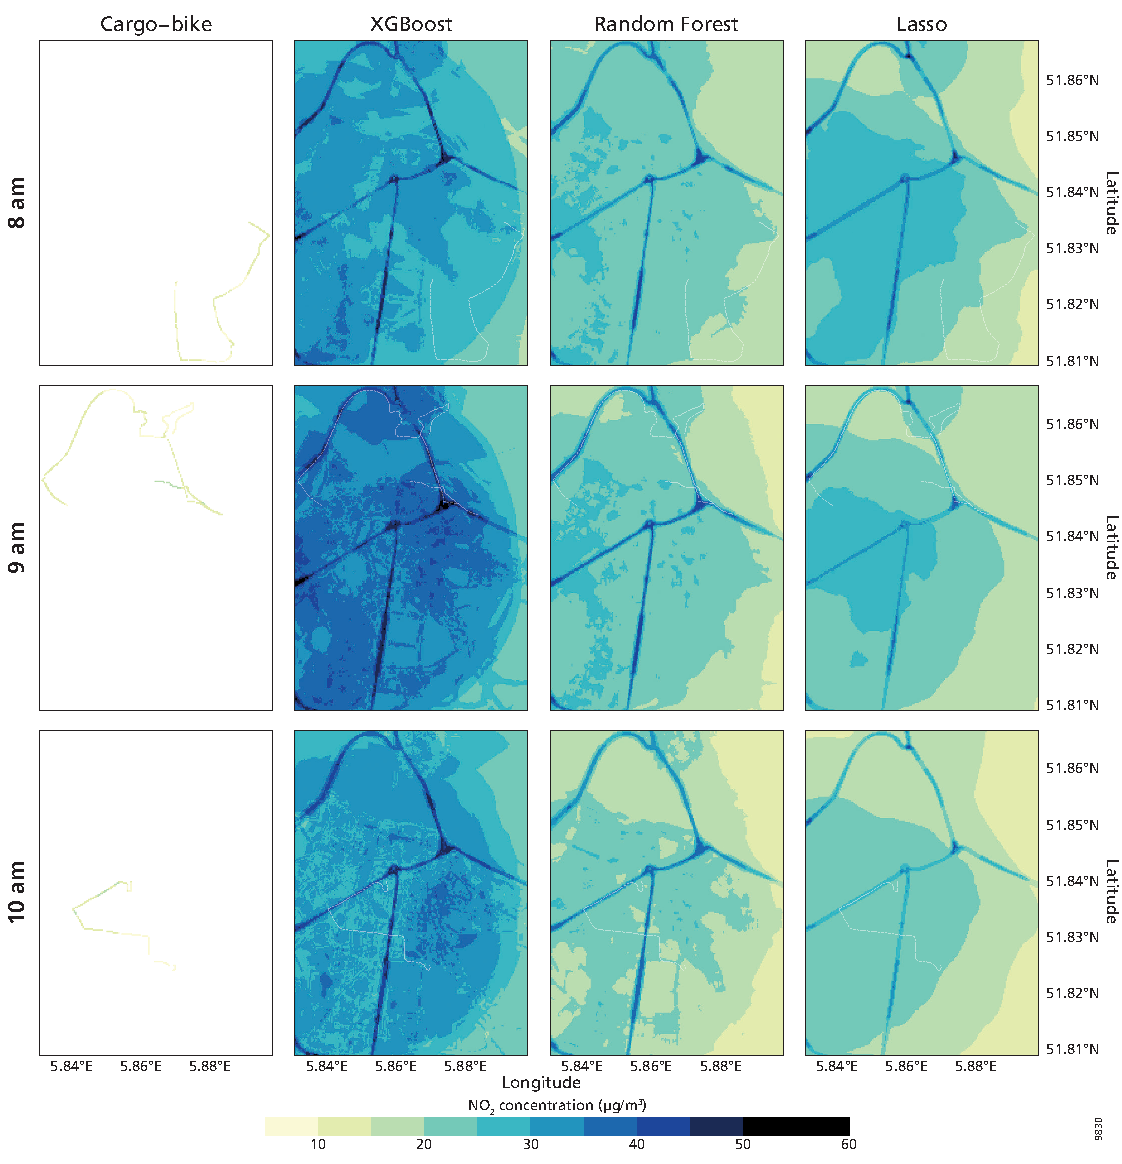
\includegraphics[width=\linewidth]{maps.pdf}
    
    \caption {Maps of cargo-bike measurements and predictions from XGB,  RF,  Lasso, hourly models. The dashed lines in the prediction maps indicate the cargo-bike routes.}
    \label{maps}
\end{figure}



\begin{figure}[H]
    \includegraphics[scale = 0.7]{ori.pdf}
    
    \caption {Cargo-bike measurements and the XGB (high setting), RF, Lasso predictions and the cargo-bike measurements, visualised in the 1-D view. The point\_id on the x-axis refers to the position on the track followed by the cargo bike.}
    \label{ori1d}
\end{figure}

 \begin{table}[H] \centering 
  \caption{mean NO$_2$ of cargo-bike, XGB, RF, Lasso, high-setting XGB (XGB hs)and cargo-bike measurements.} 
    \label{mean} 
\begin{tabular}{@{\extracolsep{5pt}} cccccc} 
\\[-1.8ex]\hline 
\hline \\[-1.8ex] 
 
Time &Cargo-bike &XGB & RF & Lasso &XGB hs \\
\hline \\[-1.8ex] 
8 am  & 10.5 &22.3& 22.3 & 22.6 & 21.6  \\
9 am & 11.4 &25.1& 16.0 & 17.1 & 21.2\\
10 am& 11.2 &30.6& 20.0 & 19.2 & 18.7\\
\hline \\[-1.8ex] 
\end{tabular} 
\end{table}   

\begin{figure}[H]
    \includegraphics[scale = 0.7]{fitted.pdf}
    
    \caption {Cargo-bike measurements and the fitted values of a linear regression between respectively the XGB (high setting), RF, Lasso predictions and the cargo-bike measurements, visualised in the 1-D view. The point\_id on the x-axis refers to the position on the track followed by the cargo bike.}
    \label{a1d}
\end{figure}




\begin{table}[H] \centering 
  \caption{$R^2$ between each RF, Lasso, high setting of XGB (XGB hs) and cargo-bike measurements.} 
    \label{r2bf} 
\begin{tabular}{@{\extracolsep{5pt}} cccc} 
\\[-1.8ex]\hline 
\hline \\[-1.8ex] 
 
Time   & RF & Lasso & XGB hs \\
\hline \\[-1.8ex] 
8 am    & 0.02 & 0.00  & 0.27\\
9 am   & 0.16 & 0.1 & 0.09\\
10 am  & 0.52 & 0.58  & 0.50\\
\hline \\[-1.8ex] 
\end{tabular} 
\end{table} 



%\begin{figure}[H]
 %   \includegraphics[width=\linewidth, trim=1cm 4cm 0cm 1cm, clip=true]{diffsgbhs.pdf}
    
%    \caption {Differences in NO$_2$ ($\mu g/m^3$) between the high-setting XGB model predictions and the cargo-bike measurements (cargo-bike measurements \textit{minus} the model prediction), at different hours. }
%    \label{diffxgbhs}
%\end{figure}
 

 
\section{Discussion}
 
% add Bakfiets error sources 
 
In this study, we used a cargo-bike with various air quality sensors and high-end instrumentation for gathering spatially more detailed ground validation data. The high-end monitors we used are equivalent to those used for official air quality monitoring. With high-end monitors, i.e. apparatus, we can measure as accurate as reasonably possible in (most) circumstances, not or minimally affected by temperature, humidity and other cross-reactivity (e.g., NO$_2$ sensors can be cross reactive to NO and O$_3$). As these monitors are usually quite large (19” rack form factor or comparable), until now this equipment (as far as we know) has only been used stationary or on a car or van. With the cargo-bike we could reach considerably more areas in a city, still using this high-end equipment. High-end equipment on board a cargo-bike gives the possibility to measure right at the place of interest such as densely populated areas (e.g., city centre) or where events occur.

With our unique cargo-bike dataset, this study provides a strong indication that the hyperparameter optimisation and model evaluation results based solely on CVGS may be misleading. In this study, the XGB and RF models with hyperparameters optimised based on k-fold CVGS obtained similar modelling CVGS accuracy. However, a comparison of spatial patterns in NO$_2$ predictions and cargo-bike NO$_2$ measurements as well as the validation of predictions against cargo-bike data indicate the RF model is more favourable. Using a lower learning rate for the XGB gives similar CVGS results compared to RF, but very different and seemingly more detailed spatial prediction patterns. The cargo-bike measurements provide a quantitative measure to understand which model gives the most realistic spatial predictions, and in our study this was the high-setting XGB model. The conventional CVGS-based model evaluation and hyperparameter optimisation lack this information and may lead to wrong conclusions regarding model comparison. We demonstrated that it is important to consider spatial prediction patterns when evaluating model predictions of NO$_2$. In addition, we have shown that spatially-continuous measurements are a valuable source of information to improve the hyperparameter tuning and model evaluation. Importantly, external measurements provide us with an objective, quantitative measure to involve the spatial prediction pattern in the hyperparameter tuning and modelling processes. 

The route track taken at the 8 am by the cargo-bike are mostly far away from major traffic roads (further than 500 m away from "primary roads" defined by OpenStreetMaps), and the route track taken at 9 - 10 am and 10 - 11 am are mostly in a traffic area. Among the prediction models, XGB hs obtained the highest $R^2$ with the cargo-bike measurements at 8 am, which shows the least variations compared to other times (\cref{ori1d}). This may indicate that the XGB is less prone to over-fitting when its hyperparameters are properly set. The best match between all the models and the cargo-bike measurements is at 10 am. This indicates that the statistical models are capable of capturing the traffic emission related variations. There is an inconsistency between the R$^2$ of CVGS (\cref{nlde_cv}, i.e. the lowest for Lasso and for 10 am) and when comparing with the cargo-bike measurements (\cref{r2bf}, the highest for Lasso and 10 am). This may be due to the fact that the cargo-bike can better capture local variations. Future studies need to include traffic volumes to better understand the amount of local variations that could be captured with statistical models. 

The hyperparameter that affects the prediction pattern of XGB the most is the learning rate. In this study, reducing the learning rate led to a clearer pattern and is closer to the cargo-bike measurements. Moreover, other model over-fitting controlling strategies, such as increasing gamma, lambda, and reducing sub-sampling do not considerably alter the prediction patterns or the CVGS accuracy, which may indicate that the model is not subject to over-fitting.  
%These results are surprising as these factors are believed to be at least alter the spatial prediction pattern more than just subtle, if not the CVGS accuracy.        


An important difference between the validation on cargo-bike and CVGS is that the CVGS measurements include all scales of spatial variations (short range, medium range, large range), while the cargo-bike measurements include only local variations. This means testing with CVGS evaluates the model also on its capability to predict large scale patterns, while testing on the cargo-bike measurements mainly evaluates the model on its capability to predict detailed local variations. A model trained on a data set that includes all scales of variation (CVGS) does not necessarily need to be the model that performs best when mapping the detailed local variations.

\section{Conclusion}
In this study, we designed a novel tool to measure detailed NO$_2$ along the roads and used the measurements to further evaluate and compare high-resolution statistical NO$_2$ models.  The spatially continuous measurements from the cargo-bike allow us to compare different statistical methods and hyperparameter settings accounting for their spatial patterns. This is complementary to the CVGS-based accuracy assessment. As the ground truths are scattered, almost all the current NO$_2$ model comparison studies ignore the spatial prediction patterns in hyperparameter optimisation and model evaluation. With advanced sensor techniques, this study provides a more thorough approach for NO$_2$ model evaluation and highlights the possible pitfall of exclusively depending on CVGS accuracy in model hyperparameter optimisation and comparison. We conclude in this study that the XGB is the most suitable for high-resolution NO$_2$ mapping compared to RF and Lasso as it is the most robust against over-fitting. The differences between XGB and RF are however not considerable and they are both better than Lasso. While the CVGS accuracy stays the same, the predictions from XGB can vary greatly with different hyperparameter settings, particularly the learning rate.    


\section*{Acknowledgement}
This research is funded by the Global Geo Health Data Centre (Utrecht University) and the Startimpulsprogramma Meten en Detecteren van Gezond Gedrag (Dutch Science Foundation). We are thankful to Evert Duistermaat, who cycled the cargo-bike and Sieger Henke, who contributed with practical, coordination and some scientific works. The authors appreciate Ton Markus for his advises and contributions on improving the figures. The authors are grateful to the editors and reviewers for their contributions. 

\newpage
\bibliographystyle{plainnat}
\bibliography{ref}

\end{document}
